\documentclass[runningheads,a4paper]{llncs}

\usepackage{amssymb}
\setcounter{tocdepth}{3}
\usepackage{graphicx}
\usepackage{amsmath}
\usepackage{verbatim}
\usepackage[margin=0.9in]{geometry}
\usepackage{amsfonts}
\usepackage{subfigure}
\usepackage{mathtools}
\usepackage{float}
\usepackage{caption}
\usepackage{subcaption}
\usepackage{cite}
\usepackage{hyperref}
\usepackage{url}
\urlstyle{same}
\newcommand{\keywords}[1]{\par\addvspace\baseline skip
\noindent\keywordname\enspace\ignorespaces#1}
\newcommand{\x}{\overline{x}}
\newcommand{\fc}{\frac{x_C}{N}}

\setcounter{secnumdepth}{5} 

\makeatletter
\let\c@lemma=\c@theorem
\let\c@corollary=\c@theorem
\let\c@fact=\c@theorem
\makeatother

%\let\realendproof=\endproof
%\def\end proof{\hspace*{\fill}$\Box$\realendproof}
\date{October 29th, 2014}							% Activate to display a given date or no date 

\begin{document}

\title{The NP-Completeness and ASP-Completeness of Some Paper and Pencil Puzzles}
\titlerunning{}

\author{Fermi Ma \and Ariel Schvartzman \and Erik Waingarten}
%
\authorrunning{Fermi Ma \and Ariel Schvartzman \and Erik Waingarten}
% (feature abused for this document to repeat the title also on left hand pages)

% the affiliations are given next; don't give your e-mail address
% unless you accept that it will be published
\institute{Massachusetts Institute of Technology}

\maketitle

We summarize results about the NP-Completeness and ASP-Completeness of some classical paper and pencil puzzles. These consist of problems in which we are given a partially filled in grid. The goal is to fill in the rest of the grid while not violating a set of rules. Some popular examples include Number Place (Sudoku), Latin Squares, Cross Sum (Kakuro) and Calcudoku (Ken Ken). 

There are two questions we will be interested in analyzing for all of these puzzles. The first is given a partially filled in grid, can we efficiently find a solution? The answer to this question corresponds to membership in NP.
The second question is dependent on the answer to the first. If there is no efficient way to find a solution, given a solution is there an efficient way to find another solution? The answer to this question corresponds to membership in ASP. 

We assume the reader has familiarity with these classes. In particular, it is worth noting that if a problem is ASP-Complete, it is also NP-Complete. On the other hand, an NP reduction will only provide a valid ASP reduction if it is \textit{parsimonious}. 

In this paper we combine results from several papers and study the connection between these puzzles and graph theoretical problems. The ultimate goal is to obtain a chain of reductions starting from a well known ASP-Complete problem and show that Number Place, Latin Squares and Calcudoku are both NP-Complete and ASP-Complete. The ASP-Completeness results follow from the fact that the NP-Completeness reductions are parsimonious. 

In section 1, we define all the we will be interested in presenting. In section 2, we introduce some edge partition problems. We show that the Edge Partition problem is NP-Complete by reducing it to 3-SAT. We will then exhibit a connection between the Triangle Partition problem, a special case, and Latin Squares. We will show that this chain of reductions is parsimonious, showing that Latin Squares is ASP-Complete. In section 3, we show a parsimonious reduction from Triangle Partition to Latin Squares, showing that it is ASP-Complete. In section 4, we present a parsimonious reduction from Latin Squares to Number Place, and show that it is also ASP-Complete. In section 5, we introduce Cross-Sum and show it is NP-Complete by reducing it to ???. In section 6, we introduce Calcudoku and show that it is NP-Complete by reducing to a special case of 3-Partition.

At the time of writing, the authors are still interested in determining whether or not Calcudoku is ASP-Complete. 

\section{Preliminaries} 

In this section we will define the puzzles. We will refer to them and their respective decision problems interchangeably. 

\textbf{Latin Squares:} In Latin Squares, we are given a $n \times n$ grid, some of whose entries have been filled in with numbers from $1$ to $n$. The goal of the game is to fill the rest of the grid with numbers from $1$ to $n$ while enforcing that no row or column repeats a number. 
\newline
\textbf{Number Place:} In Number Place, we are given a $n^2 \times n^2$ grid consisting of $n^2$ $n \times n$ bolded blocks, some of whose entries have been filled in with number from $1$ to $n^2$. The goal of the game is to fill in the rest of the grid with numbers from $1$ to $n^2$ while enforcing that no row, column or bolded square repeats a numbers. 
\newline
\textbf{Calcudoku:} In Calcudoku, we are given a $n \times n$ grid consisting of connected, bolded regions called cages. Each cage contains an elementary arithmetic operation $(+, -, \times, \div)$ and a non-negative integer. The goal of the game is to fill the grid with numbers from $1$ to $n$ while enforcing that no row or column repeats a number and that for every cage, evaluating the operation on the numbers inside the cage is equal to the value of the cage. 
\newline
\textbf{Cross Sum:} 

\section{Edge Partition problems.}

In this section, we will introduce Edge Partition problems and show that they are NP-Hard by reducing from 3SAT. We will then focus on a special case, Triangle Partition. This problem will be fundamental in our understanding of Latin Squares. 

In the Edge Partition problem EP$_n$ we are given a graph $G = (V, E)$. We want to determine if there is a partition of the edges such that each part induces a subgraph isomorphic to $K_n$. For example, if $G = K_n$ then we can always trivially partition the edge set into one part. If we are given a graph $G = (V, E)$ where the degree of any vertex is less than $n-1$, then the answer will always be no. It is worth noting that if $n = 2$ we can solve the problem in polynomial time. It is equivalent to deterring whether a graph is bipartite. Therefore, we will only focus on the cases where $n \geq 3$. 

\subsection{Proof Overview that EP$_n$ is NP-Hard}

In order to show that EP$_n$ is NP-hard, we will reduce from 3SAT. We will introduce a certain type of graph that can be partitioned in exactly 2 ways. These graphs will represent the "objects" in a 3-CNF formula: the variables, and each literal in the formula. 

We will connect the graphs by  associating vertices and edges in two graphs. By associating, we mean making two vertices from two different graphs be the "same" vertex. This connects the two graphs by making some edges be part of both graphs. The effect will be that the edge partition on one graph will induce a certain edge partition on graph the other graph. 

By making the associations correctly, we will ensure that for each clause, exactly one of the three literals in the clause has a certain partition, and if a literal graph has a certain partition, then the variable graph will have a certain partition. This will finish the reduction. 

A simple visualization of an association of edges might be the following. Suppose we have two integer lattices, $A = \mathbb{Z^2}$ and $B = \mathbb{Z^2}$. We can associate the edges of the unit square together so that the edges: 
\[ \begin{array}{c} (0,0);(1,0) \\
			     (1, 0); (1, 1) \\
			     (1, 1); (0, 1) \\
			     (0, 1); (0,0) \end{array} \]
  is the same edge in graph. Visually, this means taking the two graphs $A$ and $B$, stacking them on top of each other, and then "glueing" the unit square together in both graphs. 

\subsection{A special graph, $H_{n,p}$}

We will define a graph $H_{n,p} = (V_{n,p}, E_{n,p})$ which will act as the main gadget for the reduction from 3SAT to EP$_{n}$. The property that we want is that the graph has exactly two ways to be partitioned into edges. One partition will be the assignment of True, and the other partition will be the assignment of False. 

We will define the general graph for any $n$, but since we only need the case when $n=3$. We will let 
\[ V_{n,p} = \{ x = (x_1, x_2, ..., x_n) \in \mathbb{Z}_p^n | \sum x_i = 0 \} \]
Here we are taking vertices to be points of $\mathbb{Z}_p^n$, so we have $n$-long tuples of numbers from $0, ..., p-1$. An easy computation shows
\[ |V_{n,p}| = p^{n-1} \]
Since we can pick any $n-1$ of the coordinates, and then pick the last coordinate so that $\sum x_i = 0$ modulo $p$.

For edges, we let $(x,y)$ be an edge, if $x$ and $y$ differ only at two indices, $i,j$ and the difference between these indices is $1$. 

Note that $p$ will be an additional parameter in this graph. We will use it in two ways. The first reason is that it dictates how large the graph is, this will allow us to associate edges without risking two graphs being too close to each other and making the association of edges induce some other unwanted associations. Also, it will allow us to make the graph tripartite, which will become important in the reduction from Triangle Partition to Latin Squares.

We will go through some lemmas in order to gain an intuition as to how the structure looks and to gain some comfort in working with the graph. 

\begin{lemma}
\label{lem:translation}
Suppose $x \in V_{n,p}$, then $(v_1, v_2) \in E_{n,p}$ if and only if $(v_1+x, v_2+x) \in E_{n,p}$.
\end{lemma}

\begin{proof}
The proof is almost obvious. Suppose $v_1$ and $v_2$ differ in two incides $i,j$ where $v_1(i) = v_2(i) + 1$ and $v_1(j) = v_2(j) - 1$ and everywhere else $v_1(k) = v_2(k)$. This happens if and only if $v_1(i) + x(i) = v_2(i) + x(i) + 1$ and $v_1(j) + x(j) = v_2(j) + x(j) - 1$, and $v_1(k) + x(k) = v_2(k) + x(k)$. 
\end{proof}

Lemma~\ref{lem:translation} gives us a large amount of symmetry in the graph. In particular, it tells us that each vertex looks the same. This is because we can analyze each vertex $x$ by analyzing any translation of $x$; in particular, we can analyze the vertex at the origin. 

\begin{lemma}
\label{lem:flip}
$(v_1, v_2) \in E_{n,p}$ if and only if $(-v_1, -v_2) \in E_{n,p}$
\end{lemma}

\begin{proof}
The same argument holds as above. We can multiply every equation by $-1$ and still satisfy the equations by switching $i$ and $j$.
\end{proof}

\begin{lemma}
\label{lem:perm}
Let $\pi \in S_n$ be a permutation of $n$ elements. $(v_1, v_2) \in E_{n,p}$ if and only if $(\pi(v_1), \pi(v_2)) \in E_{n,p}$, where $\pi(v)$ acts by permuting the indices according to the permutation. 
\end{lemma}

\begin{proof}
This is also a very simple argument, since the permutation acts on both vertices equally, the two indices $i$ and $j$ are sent to some other $i'$ and $j'$ according to the permutation.
\end{proof}

Now we know that we can translate vertices and flip signs of everything, permute the indices, and still maintain isomorphic graphs. These symmetries reduce the arguments by a large amount. In particular, we will use Lemma~\ref{lem:translation}, Lemma~\ref{lem:flip}, and Lemma~\ref{lem:perm} to prove statements about the graphs by only analyzing one case. It means that when making statements about an edge in the graph, we might as well assume that edge connects the vertex at $0 = (0,0,\dots, 0)$ and a neighbor of $0$ with the first coordinate being $1$. 

\begin{lemma}
The degree of each vertex is $2\dbinom{n}{2}$.
\end{lemma}

\begin{proof}
Note that we can analyze each vertex by just analyzing the degree of $0 = (0, ..., 0)$ since we can translate by any element. We can count the neighbors of 0 by counting the indices of the coordinates where the values differ. For each $i < j \in \{ 1, ..., n\}$, we can pick either make $i = 1$ and $j = -1$, or $i = -1$ and $j = 1$. These are all neighbors of $0$. Since there are $\dbinom{n}{2}$ ways to pick ordered indices from $\{1, ..., n\}$ and each option has two possible assignments, there are $2\dbinom{n}{2}$ neighbors.
\end{proof}

\begin{lemma}
\label{lem:largestcomplete}
The largest complete subgraph is $K_n$, and any $K_3$ is contained in a unique $K_n$.
\end{lemma}

\begin{proof}
First, we show that $K_n$ is a subgraph. We can take 
\[ \begin{array}{ccccc} (0, &0, &0, &\dots, &0) \\
			     (1, &-1, &0, &\dots, &0) \\
			     (1, &0, &-1, &\dots, &0) \\
				&&\vdots \\
			     (1, &0, &0, &\dots, &-1) \end{array} \]
This subgraph is isomorphic to $K_n$. Suppose we had $K_{n+1}$ as a subgraph, we could translate the graph, flip the graph, and permute the indices of the graph in order to get the first $n$ points of the graph to be the ones listed above. Its clear to see that any other vertex will not be connected to all of them.

Now suppose we had $K_3$, with $x_1, x_2,$ and $x_3$. Then we can translate all the elements by $-x_1$, so that we are looking at $0, x, y$. Without loss of generality, we can say that the first coordinate of $x$ is 1 and there is a $-1$ at index $j$. 

So now we can look at the values of $y$ at indices $1$ and $j$. I claim that either $y(1) = 1$, or $y(j) = -1$. Suppose $y(1) \neq 1$ and $y(j) \neq -1$, then $y(1) = y(j) = 0$, since it has an edge to $0$, but then there is no edge to $y$ since there are $4$ values for which $x$ and $y$ differ. 

Once we have this, if $y(1) = 1$, $0,x, y$ sits inside the $K_n$ described above. If $y(j) = -1$, then up to a permutation of indices, $0, -x, -y$ sits inside the $K_n$ described above.
\end{proof}

We will refer to the $K_n$ has $1$'s in the same coordinate as $K$ and the $K_n$ that has $-1$ in the same coordinate as $-K$. 

\begin{lemma}
Each vertex is contained in $2n$ subgraphs isomorphic to $K_n$. 
\end{lemma}

\begin{proof}
We know that a cyclic permutation of the elements will produce disjoint $K_n$ which look like the above $K$ or like the negative of the above,  $-K$ in the Lemma~\ref{largestcomplete}. There are $n$ cyclic permutations, so there are $2n$ disjoint $K_n$ containing $0$. By Lemma~\ref{lem:translation}, we can extend this result to each vertex.
\end{proof}

\begin{lemma}
Each edge occurs in just two $K_n$.
\end{lemma}

\begin{proof}
We just need to check the edges incident on 0. Suppose the edge connects $0$ and $x$, then if the edge is a part of three distinct $K_n$, then there must be three vertices $a, b, c$ such that each one is one of the distinct $K_n$. We know that two of the three vertices $a, b$, and $c$ must be equal since either the $i$ index is the same, or the $j$ index must the same to $x$ (this follows by the same argument as in Lemma~\ref{lem:largestcomplete}). Therefore, some $K_3$ is inside two of the $K_n$, and so by the Lemma~\ref{lem:largestcomplete}, they are the same $K_n$.
\end{proof}

\begin{lemma}
Each distinct $K_n$ are either edge-disjoint, or have just one edge in common.
\end{lemma}

\begin{proof}
If there were two edges in common, then they both contain the same $K_3$, which generates the same unique $K_n$. 
\end{proof}

\begin{lemma}
\label{lem:distinctpart}
There are just two distinct edge partitions of $H_{n,p}$ into $K_n$'s.
\end{lemma}

\begin{proof}
Suppose $\Pi$ is an edge partition, and we have some edge $e$ being part of some $K_n$. Then $K_n$ looks like $K$ or $-K$ after some translation to the origin. If $K_n$ looks like $K$, then every other partition containing an edge incident on $0$ will be part of a $K_n$ that looks like $K$. Note that if it looked like $-K$, then it would share an edge. 

Since the graph is connected, there is a path from each edge to another edge. In each edge, they are incident on the same vertex. After translating each vertex to 0, its clear that all edges on the path will be part of some $K_n$ that looks like $K$, and since translation preserves signs, all edges on the path between two edges is part of a complete graph that looks like $K$. This means that every edge in the partition belongs to some $K_n$ that looks like $K$.

The same argument holds for $-K$. This means that the partition of a single $K_n$ determines the partition of the entire graph. Either it is determined by the the edge from $0$ to $(1, -1, 0, \dots, 0)$ being part of $K$, or $-K$. This means there are two ways to partition the graph.  
\end{proof}

Now we will let $T$-partitions of $H_{n,p}$ correspond to the edge $e$ connecting $0$ and $x = (1, -1, 0, \dots, 0)$ being part of $K$ and $F$-partitions of $H_{n,p}$ correspond to the edge $e$ being part of $-K$. Note that by Lemma~\ref{lem:distinctpart}, these are two mutually exclusive partitions of $H_{n,p}$.

\subsection{A Special Case: Triangle Partition}

Triangle Partition is a special case of Edge Partition that arises when we let $n = 3$. We can think of the graph as looking like perfect triangle packing of smaller equilateral triangles, with some additional edges on the sides.

\begin{figure}[h]
\label{fig:H3at0}
\centering
\includegraphics[width=0.5\linewidth]{h3at0.pdf}
\caption{$H_{3,p}$ near vertex $(0,0,0)$}
\end{figure}

We can look at what the graph looks like near the 0 vertex (see Figure~\ref{fig:H3at0}).
If we rotate to see the plane $x + y + z = 0$ on the paper, then we will get the graph with a equilateral triangle tiling of the plane. Where the shapes will look like repeating values of Figure~\ref{fig:triangletiling}.

\begin{figure}[h]
\label{fig:triangletiling}
\centering
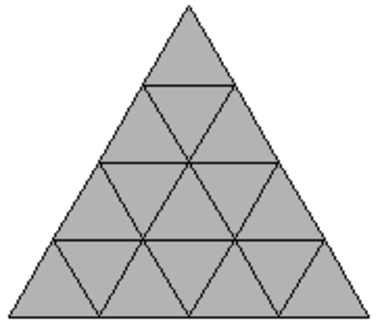
\includegraphics[width=0.2\linewidth]{EdgePartitionPic1.pdf}
\caption{Equilateral triangular tiling of the plane}
\end{figure}

Note that all side lengths are even, so when we compose these, the side lengths will be even. We can therefore, add edges on the sides by 2's and edges connecting the three points, and this will have exactly two ways of being partitioned. 

The reduction will take a big enough graph such that we can associate various triangles with each other. So we won't worry much about how we partition the ``ends" of the graph. A possible example is the following

The partition adding of the edges is shown in Figure~\ref{fig:edgecases} and their partitions are shown next to it. A green circle means that the triangle with green as the interior is a partition. The green circle not contained in any triangle signifies that the outer edges form a triangle. Note that we can increase the size of the graph by doubling the side lengths, which will mean that the exposed sides will have additional edges connecting the three new ends. 
\begin{figure}[b]
\label{fig:edgecases}
\centering
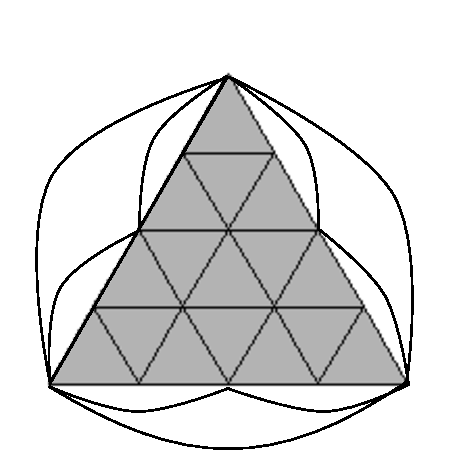
\includegraphics[width=0.2\linewidth]{triangleGraph.pdf} \qquad
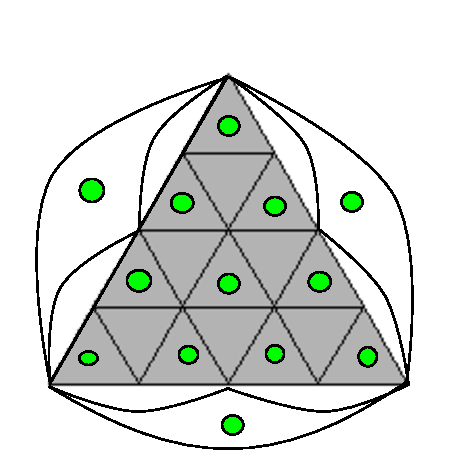
\includegraphics[width=0.2\linewidth]{triangleGraphT.pdf} \qquad
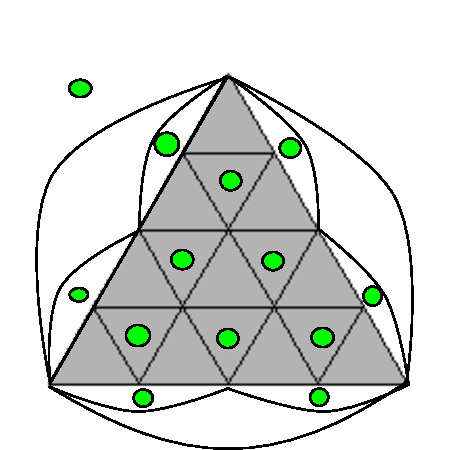
\includegraphics[width=0.2\linewidth]{triangleGraphF.pdf}
\caption{Fixing the ends of the graph and their corresponding partition}
\end{figure}

In general, $H_{n,p}$ does something similar, but with higher value cliques. The $p$ represents how tall the triangle is. 

\subsection{NP-hardness of EP$_n$.}

\subsubsection{Patch Gadgets}

Now that we understand the graph, we can reduce from 3 SAT. We will have copies of the above triangle graph that are large enough to contain many \emph{patches}. By a patch, we mean the packing of the four triangles. An $F$-patch is an upward facing patch, and a $T$-patch is a downward facing path (see Figure~\ref{fig:patches}).

\begin{figure}[h]
\label{fig:patches}
\centering
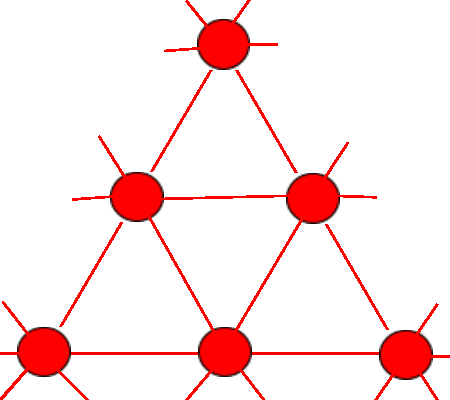
\includegraphics[width=0.2\linewidth]{Tpatch.pdf} \qquad
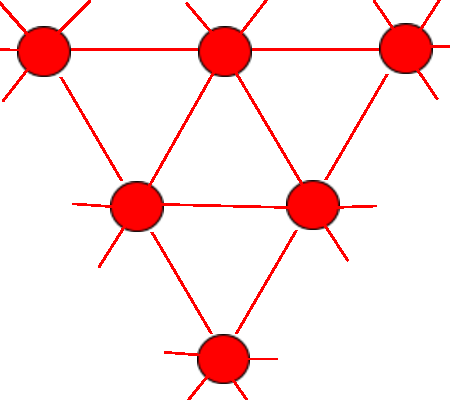
\includegraphics[width=0.2\linewidth]{Fpatch.pdf}
\caption{$F$-patch and $T$-patch}
\end{figure}

We will call a partition of a graph a \emph{$T$-partitioned} if every $T$-patch is partitioned into 3 triangles. We will call a partition of a graph an \emph{$F$-partitioned} if every $F$-patch is partitioned into $3$ triangles. Therefore, an $F$-partition will look like the middle partition in Figure~\ref{fig:edgecases}, and a $T$-partition will look like the left partition in Figure~\ref{fig:edgecases}.

\begin{definition}
In two $T$-patches or two $F$-patches, $P_1$ and $P_2$, vertices $v_1 \in P_1$ and $v_2 \in P_2$ correspond if $v_1$ and $v_2$ are in the same relative position. In a $T$-patch $P_1$ and an $F$-patch $P_2$, $v_1$ and $v_2$ correspond if they are in the same relative position after a rotation of 180 degrees.
\end{definition}

This definition corresponds the obvious elements. Two $F$-patches will have the topmost elements corresponding, the leftmost elements corresponding, and the rightmost elements corresponding. 

\subsubsubsection{Associations}

We will define an association of the graph that will have certain usefull properties. We will later use these associations to transfer information between the gadgets in the reduction. The definitions will be slightly technical. The main idea is fairly straight forward. The main idea is that we will take two graphs, and we will associate two vertices from each graph as one vertex. 

\begin{definition}
Let $G_1 = (V_1, E_1)$ and $G_2 = (V_2, E_2)$. Suppose $A \subset V_1 \times V_2$ such that
if $(v_1, v_2) \in A$, then if $(v_1, x) \in A$, $x = v_2$ and if $(x, v_2) \in A$, then $x = v_1$. Then $A$ is a valid association set of $G_1$ and $G_2$. 
\end{definition}

We require this definition so that we are associating one vertex from each graph. For our purposes, we don't need to make any more complicated associations.

\begin{definition}
Suppose $G_1 = (V_1, E_1)$, $G_2 = (V_2, E_2)$ and $A$ be a valid association set of $G_1$ and $G_2$, then let $\pi: V_1 \cup V_2 \rightarrow V_1 \cup V_2$ where
\[ \pi(v) = \left\{ \begin{array}{cc} v_1 & \text{if } v \in V_2 \text{ and } (v_1, v) \in A \\
							v & \text{ otherwise }
						      \end{array} \right. \]
and we let $V_1 \cup V_2 / A = \pi(V_1 \cup V_2)$.
\end{definition}

\begin{definition}
We let $G'$ be the association of $G_1$ and $G_2$ according to a valid association set $A$ with vertex set $V'$ and edge set $E'$ where:
\begin{itemize}
\item $V' = (V_1 \cup V_2) / A$
\item $(a,b) \in E'$ if $\pi^{-1}(a) \times \pi^{-1}(b) \cap (E_1 \cup E_2) \neq \emptyset$
\end{itemize}
We write $G' = G_1 \cup G_2 / A$.
\end{definition}

The definition for the edge set $E'$ is a bit dense. The imporant thing to note is that an edge is included in the association if it was an edge of the graphs associated. This ensures that the graph does not introduce multiple edges. The association does exactly what we want it to do: it takes two graphs $G_1$ and $G_2$ and tuples of vertices with one from each graph, and it ``glues" the vertices according to the tuples. 

Take the following simple example. Let $G_1 = (V_1, E_1)$ be a chain of $n$ elements. So $V_1 = [n]$ and $(i, i+1) \in E_1$. Likewise, we will let $G_2$ be a chain of $m$ elements. So $V_2 = [m']$ and $(i', (i+1)')\in E_2$ (note that we used primes so that the sets are disjoint). Then if we let $A = \{ (0, 0') \}$, we will have $G' = G_1 \cup G_2 / A$ with a chain of length $n+m$. If we let $A = \{ (n-1, m-1), (n-2, m-2) \}$, we will have $G' = G_1 \cup G_2 / A$ be two chains which come together for one edge, and then seperate again for one edge each (see Figure~\ref{fig:assocationexample}).

\begin{figure}[ht]
\label{fig:associationexample}
\centering
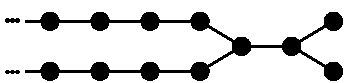
\includegraphics[width=0.5\linewidth]{associationchainexample.pdf}
\caption{Two chains assocated at one edge}
\end{figure} 

\begin{lemma}
\label{lem:varF}
Let $G_1 = H_{3, p}$ and $G_2 = H_{3, p}$ where $p$ is a large constant. Let $P_1$ be an $F$-patch in $G_1$ and $P_2$ be an $F$-patch in $G_2$. Let $A$ be the set of tuples of elements from $P_1$ and $P_2$ which correspond. Let $\Pi$ be a partition of $G_1 \cup G_2 / A$ into triangles. If $\Pi$ on $G_1$ is an $T$-partition, then $\Pi$ on $G_2 - P_2$ is a $F$-partition.
\end{lemma}

\begin{proof}
If $\Pi$ on $G_1$ is a $T$-partition, then $P_1$ will be contain only one triangle in the partition. Which means that the edges on the outside of $P_1$ will be part of triangles in the neighboring $T$-patches. So the partition of $G_2$ will be indistinguishable as if $P_2$ were a $F$-partition. And since one $F$-patch determines the partition of the whole graph, $\Pi$ on $G_2$ is $F$-partitioned.  

Figure~\ref{fig:Tpatchpartitioned} shows the $F$-patch $P_1$. The green edges corresponds to the triangle belonging to the $T$-partition of $G_1$. Also, the black edges are part of triangles of the neighboring $T$-patches on $G_1$. Therefore, to any patch in $G_2$, $P_2$ might as well have had $3$ triangles in it.
\end{proof}

\begin{figure}[t]
\label{fig:Tpatchpartitioned}
\centering
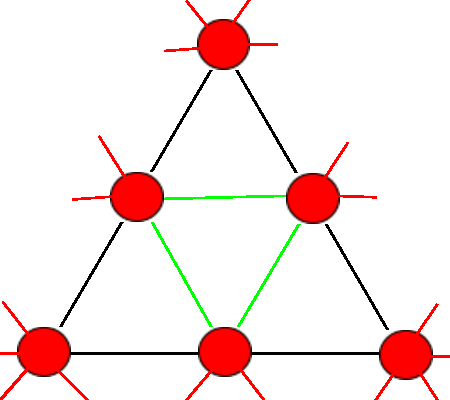
\includegraphics[width=0.2\linewidth]{TpatchPartitioned.pdf}
\caption{$G_2$ partition indistinguishable $F$-patch}
\end{figure}

Note that this proof also shows that a triangle partition after the association exists.

\begin{corollary}
\label{cor:varT}
If we associate an $F$-patch, $P_1$, of $G_1$ with an $T$-patch, $P_2$, of $G_2$, then if $\Pi$ on $G_1$ is a $T$-partition, then $\Pi$ on $G_2-P_2$ is an $T$-partition.
\end{corollary}

\begin{proof}
The same proof holds, except since we are flipping the patch, the partition of $G_2$ is inverted.
\end{proof}

\begin{lemma}
\label{lem:clause}
If we associate three graphs $G_1 = H_{3,p}$, $G_2 = H_{3,p}$, and $G_3 = H_{3,p}$ at some $F$-patch, and we remove the inner triangle of the $F$-patch, then in an edge partition of triangles, exactly one of the graphs must be a $T$-partition, and the rest must be an $F$-partition.
\end{lemma}

\begin{proof}
If we associate three $F$-patches and we remove the middle triangle, then the outer edges of the $F$-partition must be part of triangles for $T$-partitions of some graph. This means that one graph must be $T$-partitioned. The following the same arguments of Lemma~\ref{lem:varF}, the other graphs must be $F$-partitioned.
\end{proof}

\subsubsection{Proof that EP$_3$ is NP-Hard.}

\begin{theorem}
EP$_3$ is NP-hard.
\end{theorem}

\begin{proof}

The reduction is from 3SAT. Let's say $\phi$ is a 3-cnf formula with $n$ variables and $c$ clauses. We will have one graph $H_{3,p}$ for each variable, and one graph $H_{3,p}$ for each literal of each clause. 

We will choose $p$ to have a large enough graph. We want there to be many $T$-patches and $F$-patches. We also want that these patches be far away from each other, so that the associations do not interfere. In particular, we want there to be at least $3c$ patches, where $c$ will be the number of clauses in the 3-cnf formula. We can require that the distance between each patch (in a graph theoretic sense) is at least 10. Therefore, if we let $p > 30c$, we will have a large enough graph. 

So now what we will have one $H_{n,p}$ for each variable, and three for each clause. We call $U_i$ the graph $H_{3,p}$ of variable $u_i$ and $C_{i,l}$ the graph $H_{3,p}$ of the $l$th literal of the $i$th clause. If the $l$th literal of clause $i$ is $u$, then we associate a $F$-patch of $C_{i,l}$ to an $T$-patch of $U_i$. If $\overline{u}$ is the $l$th literal of clause $i$, then we associate an $F$-patch to an $F$-patch of $U_i$. 

Also, we associate three $F$-patches with each other for each $C_{i, 1}, C_{i,2}$ and $C_{i,3}$. By Lemma~\ref{lem:clause}, exactly one of the three graphs $C_{i,l}$ will be a $T$-partition, and the other two will be $F$-partitions. Suppose $C_{i,l}$ is a $T$-partition, if the $l$th literal of clause $i$ is $u$, then $U_i$ will be a $T$-partition by Corollary~\ref{cor:varT}, and if the $l$th literal of clause $i$ is $\overline{u}$, then $U_i$ will be an $F$-partition by Lemma~\ref{lem:varF}.

Therefore, if the 3SAT formula has a satisfying assignment, then we make $U_i$ be a $T$-partition if $u$ is true, and an $F$-partition if $u$ is false. Then we make $C_{i,l}$ a $T$-partition if the $l$th literal is set to true and $C_{i, j}$ for $j < l$ is an $F$-partition. This will be a valid edge partition of the graph into triangles. 

If there is a valid edge partition into triangles, then exactly one of $C_{i,l}$ is a $T$-partition for each $i$, which means that at least one literal is set to true. So we let variable the $i$th variable be true if $U_i$ is a $T$-partition, and false otherwise. 
\end{proof}

\section{Latin Squares}

In this section, we will use the result that EP$_3$ is NP-Complete in order to show the same is true for Latin Squares. After that, we use techniques by Hall [citation 5 in this pper] and Ryser [citation 13] to reduce Triangle Partition of tripartite graphs to completion.

\subsection{The Defect Graph}

Given a partial Latin square $P$ of order $n$, a \emph{defect} of the latin square is the graph $G(P) = (V,E)$ where

\begin{align*}
V = &\{r_i | \text{ row }i\text{ contains an empty square}\} \\
&\cup \{c_j | \text{ column }j\text{ contains an empty square}\} \\
&\cup \{e_k | \text{ element }k\text{ appears in fewer than }n\text{ squares}\}
\end{align*}

and

\begin{align*}
E = &\{(r_i,c_j) | \text{ the }(i,j)\text{ square of }P\text{ is empty}\} \\
&\cup \{(r_i,e_k) | \text{ row }i\text{ does not contain element }k\} \\
&\cup \{(c_j.e_k) | \text{ column }j\text{ does not contain }k\}
\end{align*}

This defect graph is a tripartite graph that has a triangle-partition if and only if $P$ is a Latin square that can be completed.

\subsection{Latin Frameworks}

In this section, we introduce the idea of a Latin framework for a tripartite graph. The intuition is as follows: under certain constraints, the Latin framework of a graph is a partial Latin square such that the original graph is the defect of this Latin square.

Given a tripartite graph $G = (V,E)$ with tripartition $V_1 \cup V_2 \cup V_3$, we label the vertices in $V_1$ as $r_1,r_2,\dots,r_{|V_1|}$, the vertices in $V_2$ as $c_1,c_2,\dots,c_{|V_2|}$, and the vertices in $V_3$ as $e_1,e_2,\dots,e_{|V_3|}$. It does not matter which vertex in each $V_i$ gets which label.

A Latin framework for such a $G = (V_1 \cup V_2 \cup V_3,E)$, denoted $LF(G;r,s,t)$ is an $r \times s$ array where each entry is either empty, or in the set $\{1,2,\dots,t\}$. Each row and column contains each element at most once, and the following additional constraints must be satisfied by $LF(G;r,s,t)$:

\begin{enumerate}
\item If $G$ contains the edge $(r_i,c_j)$, the $(i,j)$ entry is empty. If the edge is not present, the $(i,j)$ entry must be filled with an element from $\{1,2,\dots,t\}$
\item If $G$ contains the edge $(r_i,e_k)$, row $i$ does not contain $k$.
\item If $G$ contains the edge $(c_j,e_k)$, column $j$ does not contain $k$
\end{enumerate}

Observe that when $r = s = t$, $G$ is the defect of $LF(G;r,r,r)$.
We now give the following results.

\begin{lemma} 
For $G = (V_1 \cup V_2 \cup V_3,E)$, there exists a Latin framework $LF(G;n,n,2n)$ where $n = |V_1| + |V_2| + |V_3|$.
\end{lemma}

\begin{proof}
We let $LF(G;n,n,2n)$ be the $n \times n$ array where the $(i,j)$ entry is empty if $(r_i,c_j \in E)$, and contains $1 + n + ((i+j) \mod n)$ if $(r_i,c_j \not\in E)$.
\end{proof}

\begin{lemma} 
Given a Latin framework $LF(G;n,k,2n)$ where $n \leq k \leq 2n$, we can extend this to a Latin framework $LF(G;n,k+1,2n)$.
\end{lemma}

\begin{proof} 
See appendix
\end{proof}

\begin{theorem} 
For $G = (V_1 \cup V_2 \cup V_3,E)$, there exists a Latin framework $LF(G;2n,2n,2n)$ where $n = |V_1| + |V_2| + |V_3|$.
\end{theorem}

\begin{proof}
We use Lemma 1 to write down $LF(G;n,n,2n)$. We use a repeated application of Lemma 2 to add $n$ columns to get $LF(G;n,2n,2n)$, and then we transpose the machinery from Lemma 2 to add $n$ rows to get $LF(G;2n,2n,2n)$.
\end{proof}

\subsection{Solving Partial Latin Squares is NP-Complete}

We consider the problem of finding triangle partitions in a tripartite graph. First, we make the following observation about this problem. Call a tripartite graph uniform if every node has an equal number of neighbors in each of the other two partitions. A tripartite graph does not have a triangle partition if it is not uniform.

\begin{theorem}
Deciding whether a partial Latin Squares can be completed is NP-complete. Moreover, the reduction is parsimonious implying that Latin Squares is ASP-Complete
\end{theorem}

\begin{proof}
Membership in NP follows from the fact that the completed Latin square can be used as a certificate that a partial Latin square can be completed.

It remains to show NP-hardness. We do this via reduction from the triangle partition problem. Given a tripartite graph $G$, we first check whether or not it is uniform. If it is not uniform, then there does not exist a triangle partition. If it is uniform, we use Theorem 3 from the Latin frameworks section to write down a latin framework $LF(G;2n,2n,2n)$ in polynomial time. Since the Latin framework is constructed so that $G$ is a defect of $LF(G;2n,2n,2n)$, there is a triangle partition of $G$ if and only if we can complete the partial latin square $LF(G;2n,2n,2n)$. This completes the proof.

We claim that the above proofs can give us an ASP-hardness result for completing a partial Latin square. To see this, note that the triangle partitions of a defect graph $G(P)$ are in one to one correspondence with the solutions to the Latin square $P$.

\end{proof}

\section{Number Place}

In this section we show  a proof (due to Yato and Seta) that Number Place is NP-Complete and ASP-Complete by exhibiting a parsimonious reduction from Latin Squares. We will present a mapping from partially filled Latin Squares of size $n$ to partially filled in Number Place of order $n$.

Before showing the main result, we will exhibit a particular way to fill a Number Place puzzle. Next, we will show how this particular solution can be related to Latin Squares. Finally, we will show an explicit mapping from an instance of Latin Square to one of Number Place. For simplicity, throughout this argument we will be using numbers in the range $0$ through $n^2 - 1$. We will refer to the entry on the $i$-th row and $j$-th column of a Number Place puzzle as $S(i,j)$.

\begin{proposition}
Let $S_0$ be defined as
$$S_0 (i,j) = ((i \mod n) n + \lfloor i/n \rfloor + j) \mod n^2. $$
Then $S_0$ represents a solution to an order $n$ Number Place.
\end{proposition}

\begin{proof}
We will show that each column, row and block satisfy the Number Place constraints. Let $i_1 = (i \mod n)$ and $i_2 = \lfloor i/n \rfloor$. A pair $(i_1, i_2)$ uniquely represents a row or column of the Number Place. In fact, we can think of $(i_1, i_2)$ as the representation of $i$ in base $n$. This implies each number in the range from $0$ to $n^2 -1$ is uniquely represent by a pair $(i_1, i_2)$ and vice versa. In these terms, we have that
$$ S_0 (i, j) = (i_1 n + i_2 + j_2 n + j_1) \mod n^2 $$
Consider a row $i$. Suppose we have two entries such that $S(i,j) = S(i, j')$. This would imply $j_1 + n j_2 \equiv j'_1 + n j'_2 \mod n^2$. Recall that $j_1, j_2 < n$. This implies that $j = j'$. A similar argument can be applied for the columns. Consider now fixing a block by having $i_2, j_2$ fixed. Suppose we have two entries such that $S(i,j)=S(i',j')$. This means that $i_1 n + j_1 \equiv i'_1 n + j'_1$. This implies that $i_1 = i'_1, j_1 = j'_1$ and hence $(i,j) = (i', j')$. Therefore, $S_0$ defines a valid solution to a Number Place of order $n$.
\end{proof}

\begin{figure}[H]
\label{fig:S0_example}
\centering
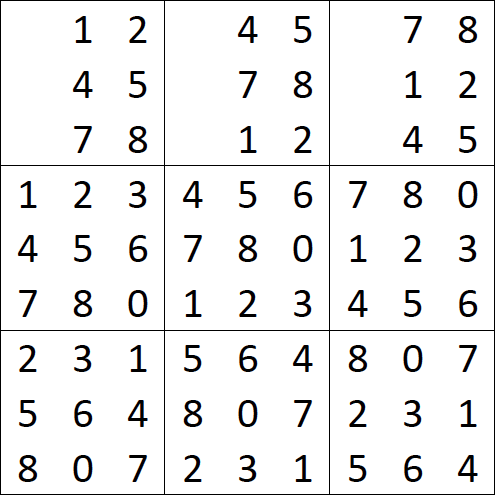
\includegraphics[scale=0.25]{sudoku-2.png}
\caption{Example of $S_0$ on a board of order 3.}
\end{figure}

\begin{lemma}
Let $S$ be a Number Place puzzle of order $n$ such that
\begin{displaymath}
S(i,j) = \left\{
\begin{array}{lr}
\perp & : (i,j) \in B\\
S_0 (i,j) & : \text{otherwise}
\end{array}
\right.
\end{displaymath}

where $B = \{ (i,j) | i < n \text{ and } (j \equiv 0) \mod n \}$. Then a square $S'$ obtained by filling in the blanks of $S$ is a solution to $S$ if and only if

\begin{itemize}
\item For any $(i,j) \in B$, $S'(i,j) \equiv 0 \mod n$
\item A square $L$ defined by $L(i, j/n) = S'(i,j)/n$ for all $(i, j) \in B$ is a Latin Square.
\end{itemize}

\end{lemma}

\begin{proof}

First of all, notice that if $(i, j) \in B$ then $j_1 = 0$ by definition. Therefore, $L(i, j/n) = L(i, j_2)$.
In this case, we only need to pay attention to the cells of $B$. We will show that the row and column constraints of a Latin Square are satisfied. From the row constraints of $S'$, we know that if $S'(i,j) = S'(i,j')$ then $j = j'$. Since we are only considering $B$ we know that $j = j' \iff j_2 = j'_2$ and $S'(i,j) = S'(i,j') \iff L(i, j_2) = L(i, j'_2)$. This ultimately shows that $L(i, j_2) = L(i, j'_2) \implies j_2 = j'_2$, which is exactly the row constraint of a Latin Square. We can argue similarly for the columns.
We can also show that the block constraints of $S'$ do not add complexity to the problem. In fact, they are equivalent to the column constraints. Therefore, the proof follows.

\end{proof}

\begin{figure}[H]
\label{fig:S_example}
\centering
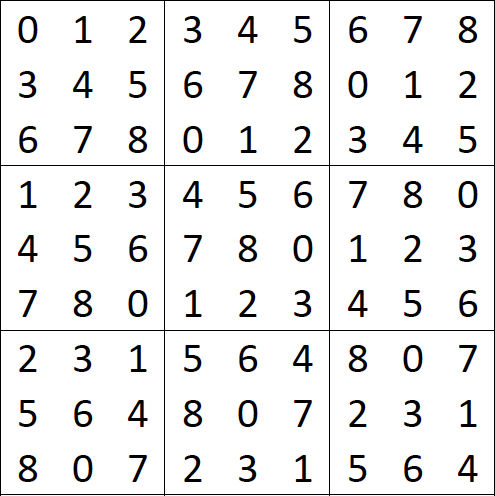
\includegraphics[scale=0.25]{sudoku-4.png}
\caption{Example of $S$ on a board of order 3.}
\end{figure}

We are now ready to show the main results of this section.
\begin{theorem} Finding a solution to an instance of Number Place is ASP-Complete. \end{theorem}

\begin{proof} We will show an ASP reduction from Latin Squares and argue that it can be done in polynomial time.
Suppose we are given a Latin Square $L$ of order $n$. We will construct a Number Place instance of order $n$ as follows:
\begin{displaymath}
S(i,j) = \left\{
\begin{array}{lr}
\perp & : (i,j) \in B, L(i, j/n) = \perp \\
L(i, j/n) n & : (i,j) \in B, L(i, j/n) \neq \perp \\
S_0 (i,j) & : \text{otherwise}
\end{array}
\right.
\end{displaymath}
This construction can be done in polynomial time. In addition, from our previous analysis we know that any solution of $L$ has a unique corresponding solution of $S$. Therefore, we get a polynomial time ASP reduction.
\end{proof}

\begin{figure}[H]
\label{fig:sudok}
\centering
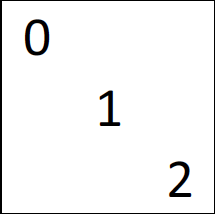
\includegraphics[scale=0.25]{sudoku-3.png}
\caption{Example of partial Latin Square of order 3.}
\end{figure}

\begin{figure}[H]
\label{fig:partialNP}
\centering
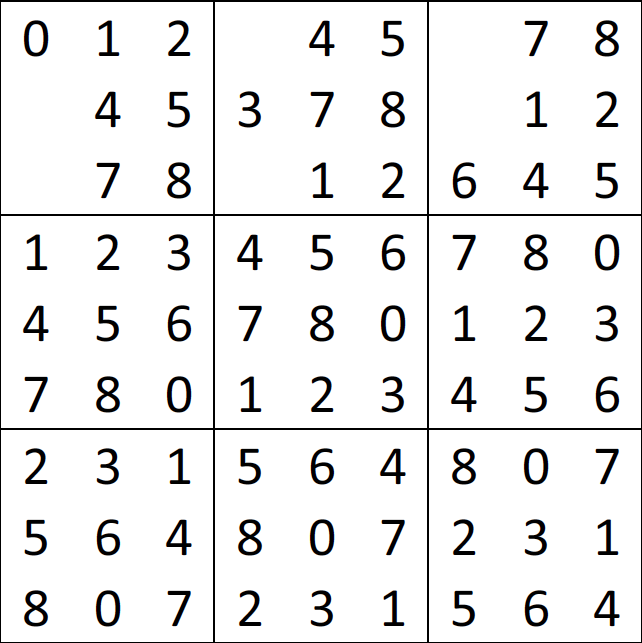
\includegraphics[scale=0.25]{sudoku-1.png}
\caption{Example of corresponding partial Number Place on a board of order 3.}
\end{figure}

\bibliographystyle{plain}
\bibliography{references}

\end{document}  
